\documentclass[12pt]{article}
\usepackage[margin=1in]{geometry}
\usepackage{graphicx}
\graphicspath{ {images/} }
\title{Lab 08: Hooke's Law and Simple Harmonic Motion}
\author{Adris Jautakas, partnered with Matthew Kendall}
\date{January 14, 2018}
\begin{document}
    \maketitle

    \pagebreak

    \section*{Abstract}
        \begin{quote}
        {\textit {\small 
            This experiment explores Hooke's Law, evaluating its accuracy through
            a series of tests involving hanging rubber bands and oscillating springs.
            We learned about the effect of mass on a spring's displacement and 
            oscillation, and discovered an unusual discrepency in our measurements
            involving the spring's spring constant that changes linearly with
            respect to mass.
        } }
        \end{quote}

    \section{Introduction}
        Hooke's law and harmonic motion describe the behavior of a spring, both
        in the force that a spring exerts and in its motion. This lab attempts
        to verify these equations by measuring the elongation of a spring and
        the period of an oscillating spring, adjusting the mass of the spring's
        weights. After performing experiments and measurements, we check
        our results by plugging them back into the equation.

    \section{Materials}
        \begin{itemize}
            \item Rubber Band
            \item Pole with horizontal bar
            \item Spring
            \item Weights (of mass 5g, 10g, 20g, 50g, and 100g)
            \item Meter stick
            \item Clips (to attach pole, horizontal bar, and meter stick)
            \item Stopwatch
        \end{itemize}
    
    \section{Methods}
        \subsection{Experiment Setup}
            The pole must first be fixated perpendicular to the ground.
            Then, a horizontal bar should be attached to the pole such that
            masses can be hung from the bar without the bar moving or falling
            off. Then there are three experiments run on this setup
        \subsection{Experiment A: Rubber Band Elongation}
            The rubber band is attached to the horizontal pole, and a weight
            is attached to the rubber band. The rubber band stretches due to
            the weight of the masses, and that stretching distance is to be
            recorded. Repeat this for varying masses.
        \subsection{Experiment B: Spring Elongation}
            Repeat the procedure in Experiment A with the rubber band, but use
            a spring and adjust the weights appropriately
        \subsection{Experiment C: Period of Elongation}
            Repeat the procedure in Experiment B, but drop the mass from a
            certain height and measure the period of oscillation. This is done
            by tracking how many times the spring system completes a full 
            oscillation over a given period of time (in this case it was 5
            seconds)

    \section{Data}
        {\large Experiment A: Rubber Band Elongation} \\
        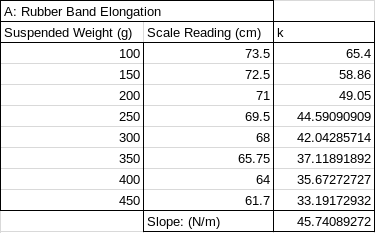
\includegraphics[scale=0.75 ]{LazyChartA.png} \\ \\
        {\large Experiment B: Spring Elongation} \\
        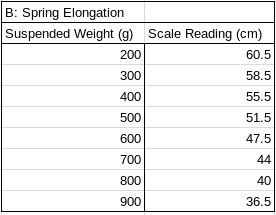
\includegraphics[scale=0.75]{LazyChartB.png} \\ \\ 
        \begin{minipage}{\linewidth} % Keeps it together without breaking
            {\large Experiment C Data: Spring Oscillation} \\ 
            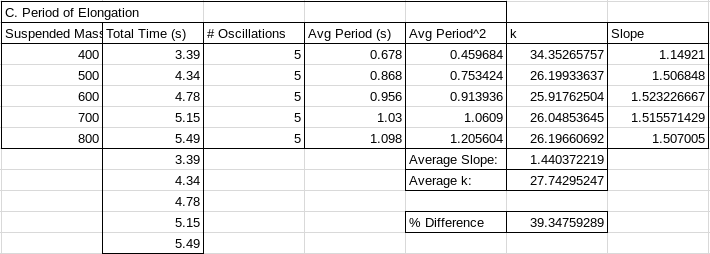
\includegraphics[scale=0.75]{LazyChartC.png} \\ \\
        \end{minipage}
        {\large Experiment C Graph: Spring Oscillation} \\
        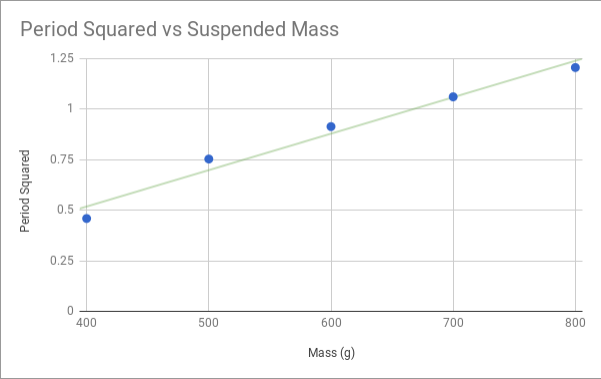
\includegraphics[width=\textwidth]{Graph1.png} \\ \\
    \section{Analysis}
        \subsection{Equations}
            Hooke's law is described as $F_s = \mu_k \Delta x$ where $F_s$ is
            the force of the spring, $\Delta x$ is the elongation of the
            spring, and $\mu_x$ is the spring constant in $N/m$ for the spring,
            controlling how aggressive or powerful it is.
        \subsection{Evaluation of Data: Spring Elongation Spring Constant}
            For the spring experiment, the spring constant for each trial can be
            determined using Hooke's Law, solving for $\mu_k$.
            $\mu_k = \frac{F_s}{\Delta x}$. The calculated slope of the spring
            graph is then defined by the average of all of all $\mu_k$'s.
        \subsection{Evaluation of Data: Period of Oscillation}
            Applying Hooke's Law to harmonic motion, we can use the equation
            $T_s = 2\pi \sqrt{ \frac{m}{\mu_k}}$ to iscolate for $\mu_k$ and 
            get $\mu_k = \frac{4pi^2m}{{T_s}^2}$. We can expect $\mu_k$ to not
            deviate too much from the experiment, and for the relationship between
            ${T_s}^2$ and $m$ to be linear. These are plotted in the graph above,
            showing a line of best fit with a slope of $1.44 \frac{s^2}{kg}$ and
            an $r^2$ deviation of 0.973 (pretty close), proving that k does in fact
            have a clear relationship with time that follows Hooke's Law.
        \subsection{Deviating $\mu_k$}
            An interesting point to note is that throughout our experiment, $\mu_k$
            deviates at a constant rate with respect to $m$: The higher the mass,
            the lower the $\mu_k$: This applies across our different experiments.
            Plotting the graph of $\mu_k$ vs $m$ reveals what appears to be a linear
            relationship up until a certain point when the mass excedes 500g.
    \section{Conclusion}
        Despite the significant error in our experiment, we've confirmed that
        surprisingly, Hooke was in fact correct and the laws of physics as we
        know them do not need to be completely rewritten. Our $\mu_k$ values
        deviated and were responsible for our error, and they deviated at a
        constant rate which suggests that there is an extra physical property at
        play. Perhaps the spring has some kind of friction or dampening that gives
        it higher resistance when it's pulled by a small ammount, making $\mu_k$
        significantly larger at short displacements.
\end{document}
